\documentclass[../CourseManual.tex]{subfiles}

\begin{document}

The second algorithm being discussed is the flocking algorithm. This algorithm is designed to find a consensus velocity that all agents within the system will travel at, causing the agents to “flock” together. This algorithm could be used to model self-driving vehicles, animal behaviour, or any situation where agents are required to stick together while traveling.

\subsection{Flocking Consensus Dynamics} \label{Flocking Consensus Dynamics}

The dynamics for the flocking algorithm are very similar to the formation algorithm, and are given by the system of differential equations

\[
\boldsymbol{\dot{v}} = - L \cdot \boldsymbol{v}.
\]

where the $n \times 2$ velocity vector, $\boldsymbol{v}$, is calculated by

\[
\boldsymbol{v} = \boldsymbol{\dot{q}},
\]

and the Laplacian matrix, L, is calculated by 
\[
L = D-A.
\]

In the case of the flocking algorithm, the adjacency matrix, $A$, is calculated differently than in the formation algorithm. Unlike formation, where agents were either in open or closed communication with another agent, agents are now assumed to be in communication with each other, but the strength of the communication between agents is dependent on the distance between agents. In the flocking algorith, the entries for the adjacency matrix are calculated by
\[
A(i,j) = \frac{K}{(\sigma^2+d^2)^\beta},
\]
%% Need to define what K, SIGMA and BETA would be in reality, RESEARCH REQUIRED.

where $K$, $\sigma$, and $\beta$ are user defined parameters. The parameter $K$ denotes a proportional gain on the communication between the two agents. The parameter $\sigma$ denotes a decrease in communication strength between agents. The parameter $\beta$ denotes the rate at which the signal strength changes over distance. Furthermore, the variable $d$ denotes the Euclidean distance between agents $i$ and $j$ and is calculated by

\[
d = ||q_i -q_j||. 
\]

The degree matrix, $D$, is calculated in the same manner as in the formation algorithm by

\[
D(i,i) = \sum_{j=1}^{n}{A(i,j)}.
\]

In order to model the algorithm, the system needs to be translated into the discrete time domain from a continuous system. In the discrete time domain, the system updates the velocity of each agent using
\[
\boldsymbol{v}(t+\Delta t) = \boldsymbol{v}(t) - L \cdot \boldsymbol{v}(t) \cdot \Delta t,
\]
where $\Delta t$ is a fixed time step. 

\subsubsection{Introducing a Leader} \label{Introducing A Leader}
A leader is a single agent that is defined to follow a specified parameterized path independent of the velocities of the other agents in the system. The purpose of introducing a leader is to have the other agents follow the leader. 

\subsubsection{Introducing a Trigger Sequence} \label{Introducing a Trigger Sequence}
A trigger sequence, $T$, is a $1\times T_{max}$ vector containing ones and zeros, where $T_{max} = \frac{duration}{\Delta t}$ is the number of iterations for which the simulation will run, and $duration$ is the length of time for which the simulation will run. With a trigger sequence, the system updates the velocity of each agent using
\[
\boldsymbol{v}(t+ \Delta t) =
\begin{cases}
    \boldsymbol{v}(t) - L \cdot \boldsymbol{v}(t) \cdot \Delta t, & \text{ if } T(t) = 1,\\
    \boldsymbol{v}(t), & \text{ if } T(t) = 0.
\end{cases}
\]

This sequence determines when the algorithm will allow the agents to communicate and update their velocities. If the time step that you set for your simulation is very small, it may not be possible or cost effective to have the agents update their velocities every iteration. You can use the trigger sequence to represent the real world limitations on the communication capabilities between agents. A possible area to explore is experimenting with the minimum number of communications your system requires to remain well connected (i.e. no rogue agents). The trigger sequence is one of the functions you will be designing for the Flocking Simulation's operation.

\subsection{Simulation App} \label{Simualtion App: Flocking}
The app provided uses the consensus dynamics defined in \hyperref[Flocking Consensus Dynamics]{Section \ref{Flocking Consensus Dynamics}} to update each agent’s location for every iteration of the simulation.  The critical components of the app's functionality have been placed in external functions, which you will develop over the course of the project. The functions that you will be responsible for are discussed in detail in \hyperref[MATLAB Functions: Flocking]{Section \ref{MATLAB Functions: Flocking}}. \\

Upon simulation completion, the app will create an excel file named \textit{agentData.xlsx} containing the positions and velocities for all agents, throughout the duration of the simulation. This data should be used to conduct further analysis to improve or validate your design.

%app picture goes before the descriptions
\begin{figure}[H]
    \centering
    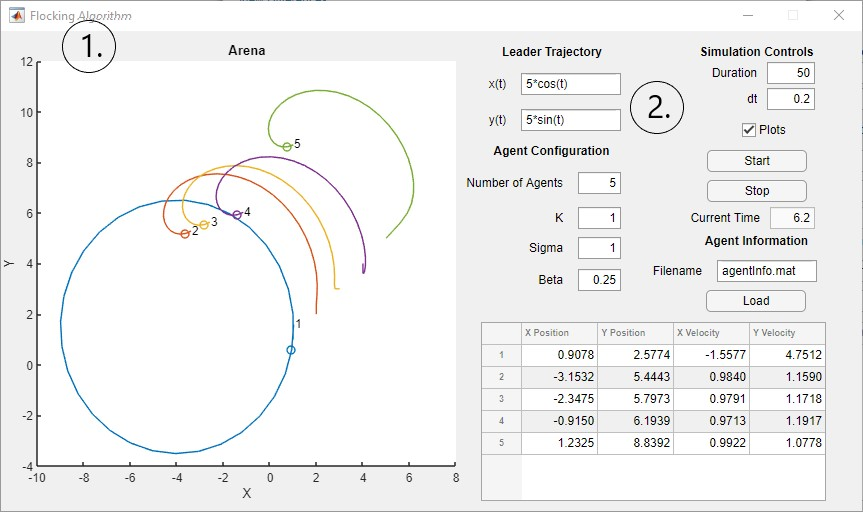
\includegraphics[width=350pt]{media/Flocking.jpg}
    \caption{Screen capture of FlockingApp.mlapp with default settings}
    \label{fig: flocking app}
\end{figure}

\subsubsection{Plots} \label{Plots: Flocking}
Area 1 of Figure \ref{fig: flocking app} displays the plots section of the Flocking app. This section contains a single plot, the \textbf{Arena} plot. \\

The \textbf{Arena} plot for the Flocking app displays the current position of each agent using a small circular marker with corresponding agent number. The coloured line trailing from each agents' current position marker indicates the path traced by that agent during the simulation thus far.  


\subsubsection{User Controls} \label{User Controls: Flocking}
Area 2 of Figure \ref{fig: flocking app} displays the user controls section of the Flocking app. This section is divided into 4 sub-sections: the \textbf{Agent Configuration} sub-section, the \textbf{Simulation Controls} sub-section, the \textbf{Leader Trajectory} sub-section, and the \textbf{Agent Information} sub-section.\\

The \textbf{Agent Configuration} sub-section is where you can enter the design parameters for the \textbf{Number of Agents}, and \textbf{K}, \textbf{Sigma} and \textbf{Beta} that are used in the adjacency matrix calculation (\hyperref[Flocking Consensus Dynamics]{see Section \ref{Flocking Consensus Dynamics}}).\\

The \textbf{Simulation Controls} sub-section contains the following commands and input windows. You can adjust the value of $\Delta t$ used in the position update equation for the flocking algorithm (\hyperref[Flocking Consensus Dynamics]{Section \ref{Flocking Consensus Dynamics}}) via the \textbf{dt} edit field. To change the length of time for which the simulation runs, adjust the value under \textbf{Duration}. The \textbf{Start} button begins the simulation and the \textbf{Stop} button stops the simulation from running. The \textbf{Plots} checkbox, when enabled, will update the \textbf{Arena} plot and the \textbf{Agent Information} table on every iteration. Disabling \textbf{Plots} will greatly increase the speed of your simulation. This is useful if you need to simulate for more than a few hundred iterations.\\

The parameterized path that the leader is to follow is entered under the \textbf{Leader Trajectory} sub-section. The parameterized equation for the $x$ position of the leader is entered in the \textbf{x(t)} window and similarly \textbf{y(t)} for the parameterized $y$ position equation of the leader. The parameterized equations must be written in terms of $t$.\\

The \textbf{Agent Information} sub-section allows parameters to be loaded from a \textit{.mat} file created using the Matrix Editor. This file will contain: the initial $x, y$ positions and velocities for each agent; the leader trajectories, $x(t)$ and $y(t)$; the proportional gain $K$; the communication noise $sigma$; the signal strength decay value $beta$. These parameters are loaded by pressing the \textbf{Load} button. Alternatively, this information can be entered directly into the app. Note that information entered directly into the app will not be saved to the \textit{.mat} file. Instead, this is done using the Matrix Editor (See \hyperref[Matrix Editor: Flocking]{Section \ref{Matrix Editor: Flocking}}) \\

\subsubsection{Matrix Editor} \label{Matrix Editor: Flocking}

The \textbf{Matrix Editor Flocking} app can be used to create a matrix that stores the initial position and velocity information for each agent. The number of agents is reflected in the number of rows of the position velocity table. Additional information can also be stored in the .mat file by entering the $x$ and $y$ parametric equations for the leader trajectory and the $K$, $sigma$, and $beta$ values in the appropriate text-boxes. The file name for the .mat file can also be altered to allow for multiple configurations to be created and stored.

\begin{figure}[H]
    \centering
    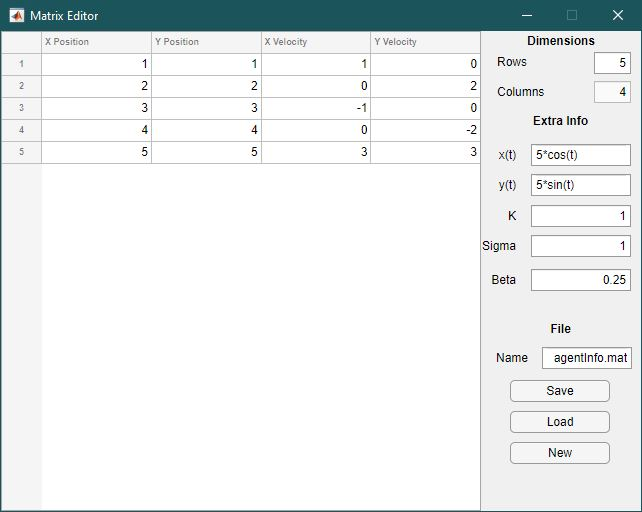
\includegraphics[width=350pt]{media/MatrixEditorFlocking.JPG}
    \caption{Screen capture of MatrixEditorFlocking.mlapp with default settings}
    \label{fig: matrix editor flocking}
\end{figure}

\subsubsection{Parameters and Variables}

\renewcommand{\labelenumi}{\roman{enumi}}
\begin{enumerate}

    \item Number of Agents $(numAgents)$: Total number of agents $(N)$ used in simulation.
  
    \item Agent Position $(agentPosition)$: An $N \times 2$ matrix with the x-position of the $i^{th}$-agent in the first column of row $i$, and the y-positions in the second column, as below:
  
    $$Agent Positions = 
    \begin{bmatrix}
    q^{1}_{x} \hspace{0.5cm} q^{1}_{y}\\
    q^{2}_{x} \hspace{0.5cm} q^{2}_{y}\\
    \vdots \hspace{0.5cm} \vdots \\
    q^{N}_{x} \hspace{0.5cm} q^{N}_{y}\\
    \end{bmatrix}$$
  
    \item K $(k)$: The parameter K is a user defined constant scalar multiplier which denotes a proportional gain on the communication between agents.
    
    \item $\sigma$ $(sigma)$: The parameter $\sigma$ is a user defined offset value which denotes a decrease in communication strength between agents.
    
    \item $\beta$ $(beta)$: The parameter $\beta$ is a user defined exponent value which denotes the rate at which the signal strength changes over distance.
    
    \item Adjacency Matrix $(A)$: The $N \times N$ adjacency matrix:
    
    $$A = \dfrac{k}{(sigma^2 + dist(i,j)^2)^{beta}}$$
    
    \item Degree Matrix $(D)$: The $N \times N$ degree matrix:
    
    \[
    D(i,i) = \sum_{j=1}^{n}{A(i,j)}.
    \]
    
    \item Laplacian Matrix $(L)$: The $N \times N$ Laplacian matrix:
    
    $$L = D - A$$
    
    \item Velocity Function $(velocityFunction)$: The $1 \times 2$ symbolic expression in terms of symbolic variable $t$ representing the parametric velocity functions $v^{L}_{x}(t)$ and $v^{L}_{y}(t)$ of the leader.
    
    $$velocityFunction = 
    \begin{bmatrix}
    v^{L}_{x}(t), v^{L}_{y}(t)
    \end{bmatrix}$$
    
    \item Duration $(duration)$: Total duration the simulation will run for.
    
    \item $\Delta t$ $(dt)$: Amount of time simulated in each iteration.
    
    \item Current Time $(time)$: Current (simulated) time.
    
    \item Leader Velocity $(leaderVelocity)$: $(duration/dt + 1) \times 2$ vector of the velocity function evaluated from $t=0$ to $t=duration$ in discrete time steps of $dt$. Hence, the resultant vector can be shown as:
    
    $$leaderVelocity = 
    \begin{bmatrix}
    v^{L}_{x}(0), \hspace{0.5cm} v^{L}_{x}(0) \\
    v^{L}_{x}(dt), \hspace{0.5cm} v^{L}_{x}(dt) \\
    v^{L}_{x}(2 \cdot dt), \hspace{0.5cm} v^{L}_{x}(2 \cdot dt) \\
    \vdots \\
    v^{L}_{x}(duration), \hspace{0.5cm} v^{L}_{x}(duration) \\
    \end{bmatrix}$$
    
    where $v^{L}_{x}(t)$ is the $x$ velocity of the leader agent at time $t$ and $v^{L}_{y}(t)$ is the $y$ velocity of leader agent at time $t$.
    
    \item Trigger Sequence $(trigger)$: The trigger sequence is a $1\times T_{max}$ vector containing ones and zeros which convey the logic for when to update agent velocities. If $trigger(t) = 1$ then the agents' velocities will be updated in following iteration. If $trigger(t) = 0$ then no velocity update will occur in the next iteration.  For more information on trigger sequences, see Section \hyperref[Introducing a Trigger Sequence]{Section \ref{Introducing a Trigger Sequence}}.
    
    \item Agent Velocity $(agentVelocity)$: The $N \times 2$ vector of agent velocities where the first column represents the $x$ velocities of agents $1$ through $N$ and the second column represents the $y$ velocities of agents $1$ through $N$ as such:
    
    $$agentVelocity = 
    \begin{bmatrix}
    v^{1}_{x}(t), \hspace{0.5cm} v^{1}_{y}(t) \\
    v^{2}_{x}(t), \hspace{0.5cm} v^{2}_{y}(t) \\
    \vdots \\
    v^{N}_{x}(t), \hspace{0.5cm} v^{N}_{y}(t) \\
    \end{bmatrix}$$
    
    where $v^{i}_{x}(t)$ is the $x$ velocity of agent $i$ at time $t$ and $v^{i}_{y}(t)$ is the $y$ velocity of agent $i$ at time $t$.
    
\end{enumerate}

\subsubsection{MATLAB Functions} \label{MATLAB Functions: Flocking}
You will need to create the following MATLAB functions in order for the simulation to function. The order that functions are listed is the order that you will be creating them during the project.\\

\textbf{calcA.m} -- calcA.m is used to calculate the adjacency matrix for the current iteration of the simulation using the user defined parameters and the agents' positions. The calcA function takes inputs $K$, $sigma$, $beta$, and $agentPosition$, and outputs $A$. $A$ is calculated as seen in \hyperref[Flocking Consensus Dynamics]{Section \ref{Flocking Consensus Dynamics}} with the equation

$$A = \dfrac{k}{(sigma^2 + dist(i,j)^2)^{beta}}$$

\textbf{calcL.m} -- calcL.m is used to calculate the Laplacian matrix for the current iteration of the simulation using the adjacency matrix. The CalcL function takes as input $A$ and outputs $L$. $L$ is calculated as seen in \hyperref[Flocking Consensus Dynamics]{Section \ref{Flocking Consensus Dynamics}} with the equation 

$$L = D - A$$

\textbf{calcLeaderVelocity.m} -- calcLeaderVelocity.m is used to calculate the velocity of the leader agent for all iterations of the simulation. Note that this function is called once at the beginning of the program, and the leaderVelocity returned should contain the leader's velocity at each discrete time step. The calcLeaderVelocity function takes inputs $velocityFunction$, $duration$, and $dt$, and outputs $leaderVelocity$. leaderVelocity is calculated by evaluating the pair of functions $\begin{bmatrix} v^{L}_{x}(t), v^{L}_{y}(t)\end{bmatrix}$ in $velocityFunction$ $\forall t \in [0, T_{max}]$ where $T_{max} = duration/dt$. \\

\textbf{trigger.m} -- trigger.m is used to calculate the trigger sequence discussed in \hyperref[Introducing a Trigger Sequence]{Section \ref{Introducing a Trigger Sequence}}. The trigger function takes as input $time$ and outputs $trigger$. $trigger$'s calculation will be determined by you over the course of the project. \\

\textbf{updateVelocity.m} -- updateVelocity.m is used to update the agents' velocities using the dynamics governed by the flocking consensus dynamics. The updateVelocity function takes inputs $L$, $dt$, and $agentVelocity$, and outputs $agentVelocity$. $agentVelocity$ is calculated as seen in \hyperref[Flocking Consensus Dynamics]{Section \ref{Flocking Consensus Dynamics}} with the equation

$$\boldsymbol{v}(t+\Delta t) = \boldsymbol{v}(t) - L \cdot \boldsymbol{v}(t) \cdot \Delta t$$

\subsection{Example: Flocking} \label{Example: Flocking}
This section provides a sample P2 project using the flocking algorithm. This example is broken down into what is to be completed each week of the project to provide a reference as to what will be expected with your project. You can not use this application area for your project.

\subsubsection{Week 1} \label{Week 1: Flocking}
\textbf{Area of Application}\\
The application area that has been selected involves some rovers following another rover through the vast expanses of Mars to conduct surveying. A new fleet of rovers is to be designed that will have 'leader' and 'follower' rovers. The 'leader' rovers with a highly accurate GPS system will be capable of effectively navigating and returning to base. The 'follower' rovers will not have GPS unit but can communicate with the leader robot. Without a leader robot, the 'follower' robots will be helpless in returning to base.\\

% A new rover is to be designed that has a highly accurate GPS that can return to the mission base solely with the use of the GPS system. The other rovers in the fleet are older models with aged components. These rovers have a radius of communication of 10 meters, can only process one communication every 60 seconds, and has no GPS system. Without the leader robot, the follower robots will be helpless in returning to the base as they will be gradually pushed off course by the uneven Martian terrain. \\

\textbf{Algorithm Selection}\\
With a potential area of application selected. The four possible group-dynamics algorithms were examined in more detail. The applicability of each algorithm was conducted to determine the most suitable algorithm for the project. Based on the application area's requirement that the agents follow a leader, the flocking algorithm was determined to be the most suitable option.\\

\textbf{Pitch Presentation}\\
With the area of application selected, a brief pitch presentation of the application area was created. This presentation provided a high-level overview of the area of application and how the group dynamics algorithms could be implemented in the design solution. 

\subsubsection{Week 2} \label{Week 2: Flocking}
\textbf{Proposal Report}\\
With the application area and flocking algorithm selected, the proposal report could then be written. This report includes the standard items listed in a design report; executive summary, introduction with background to the application area, discussion, project plan, etc. The report includes a problem definition specifying a fleet of robots that meets the desired performance abilities and satisfies the communication requirements. The main stakeholders were identified and include; the astronauts on Mars, the rover development company and the federal government or space exploration corporation. Preliminary design metrics to evaluate the effectiveness of the final design solution are also included in the report. This will involve identifying parameters in the design that can be varied. Research will be conducted to determine the various parameters and the ranges these parameters can be based on the application area.\\

\textbf{Adjacency Matrix}\\
The flocking simulation will be used to help determine if the proposed design will meet performance requirements. To model this system, a few things must be considered. First we redefine the adjacency matrix, $A$, to be:
\[
A(i,j) =
\begin{cases}
\frac{(\sigma^2 + d^2)^\beta}{K}, & \text{ if } d \leq r_c,\\
0, & \text{ otherwise.}
\end{cases}
\]

This makes it so that the agents can only communicate if they are within some set radius of communication, $r_c$, and that the signals will be stronger as the follower agent becomes farther away (this is the opposite to the default dynamics, where influence is higher as agents are closer). This models an increasing “urgency” of the signals as the follower gets farther off course. Research will need to be conducted to determine the acceptable ranges for \textit{K}, $\sigma$, $\beta$ and $r_c$. 

\subsubsection{Week 3} \label{Week 3: Flocking}
\textbf{MATLAB Coding}\\
With the adjacency matrix equation determined, it can now be translated into equivalent code to complete the \textit{calcA.m} function. In addition, the equations for determining the Laplacian matrix, $L$, can also be translated into code for the \textit{calcL.m} function. \\

\textbf{Design Process}\\
Continue establishing design metrics to be used to evaluate aspects of the final design solution. An example of one design metric will be the maximum time between communications. The longer the time between communications can be, the more cost effective the system will be by reducing the cost of the communication equipment required.\\

At this point in the project, research for Triple Bottom Line (TBL) analysis for the project; social, economic and environmental considerations should begin. This research could include; budget limits of research groups for design solution, performance, cost and environmental impact of the new robot, cost of communication equipment to be used on robots and many more. Determining how these factors will influence the design choices you make is important to keep in mind.\\

\textbf{Reports}\\
Completed the first progress report. This one-page report highlights what has been accomplished to date, what challenges the team were facing and the strategy that will be used to overcome these challenges. An outline of the team's next steps for the project should also be included.

\subsubsection{Week 4} \label{Week 4: Flocking}
\textbf{MATLAB Coding}\\
Wrote code for the \textit{calcLeaderVelocity.m} function that uses the derivative of the parametric equations describing the leader's trajectory and calculates the corresponding velocity for each iteration of the simulation. As an example, the leader's trajectory can be defined to be $v_L = (0.1t, 0.1t)$. This straight line trajectory has the leader moving at 0.141 metres per second. \\

Introduced a trigger sequence to the algorithm through the \textit{trigger.m} function to determine when the velocities of each agent will be updated. As an example, the trigger sequence is defined
\[
T(t) =
\begin{cases}
1, & \text{$t \equiv 0 \pmod{t_{update}},$}\\
0, & \text{otherwise.}
\end{cases}
\]
This establishes that the velocity of each agent is to be updated after some specified time period, $t_{update}$, between communications. This value will be varied during testing to determine the minimum number of communications required for consistent performance. The third function to be written is the \textit{updateVelocity.m} function that updates the velocity of each agent. We then account for behaviour in which a rover is navigating over uneven terrain by adding noise, $\boldsymbol{e}(t)$, to the velocities of the follower rovers
\[
\boldsymbol{v}(t) = \boldsymbol{v} + \boldsymbol{e}(t),
\]
where for each iteration $\boldsymbol{e}(t)$ is a $2 \times 1$ array of values ranging from - 0.05 to 0.05 following a Gaussian distribution.\\ 

\textbf{Design Process}\\
Developed methods to evaluate design alternatives. This could include creating an evaluation matrix. If using an evaluation matrix, be sure to justify the categories made and the weights assigned to each category (may require additional research). Energy levels within the individual rovers will be an important consideration, as they need to have returned to base before they run out of energy. This will require further research as to what factors lead to the rover's energy being depleted. Once theses parameters are determined, an energy function can be incorporated into the \textit{updateVelocity.m} function to improve the robustness of the design. Another factor to consider is that some rover movements such as accelerating/decelerating or turning could be more energy intensive. Introducing an energy function to account for this would improve simulation accuracy. These energy and cost functions will be added to \textit{updateVelocity.m} in the following week.\\

At the end of this week, the flocking simulation app is functioning and preliminary testing can begin.


\subsubsection{Week 5} \label{Week 5: Flocking}
\textbf{MATLAB Coding}\\
Based on research results, an appropriate energy and cost function can be incorporated into the \textit{updateVelocity.m} function. \\

\textbf{Design Process}\\
With the simulation now complete including the energy and cost functions, testing of the system under various parameter settings can be conducted. The ranges that various parameters can vary within have been well researched in the weeks prior. Using the design metrics established in previous weeks, the most suitable design solution can be selected. Be sure to use \textit{quantitative} design metrics when evaluating the effectiveness of a design. The evaluation of potential designs can then be compared against each other through the use of evaluation matrices, design rubrics, etc. \\

\textbf{Reports}\\
The second progress report was submitted. This one page report is similar in content and format to the progress report submitted in Week 3. Highlight any remaining challenges and/or tasks for the project.\\

Work on the final report also began detailing the Design Process, Design Solution and its justification,  TBL analysis and more. This report should include the revised sections from the proposal report based on the feedback returned.

\subsubsection{Week 6} \label{Week 6: Flocking}
\textbf{Final Design}\\
Complete any remaining tests and finalize the design specifications for the final design solution. Generate supporting materials (plots, tables, etc.) that can be used in the final report and presentation. Complete the final report and presentation for the project.


\end{document}